% Created by tikzDevice version 0.12.6 on 2026-09-28 12:30:44
% !TEX encoding = UTF-8 Unicode
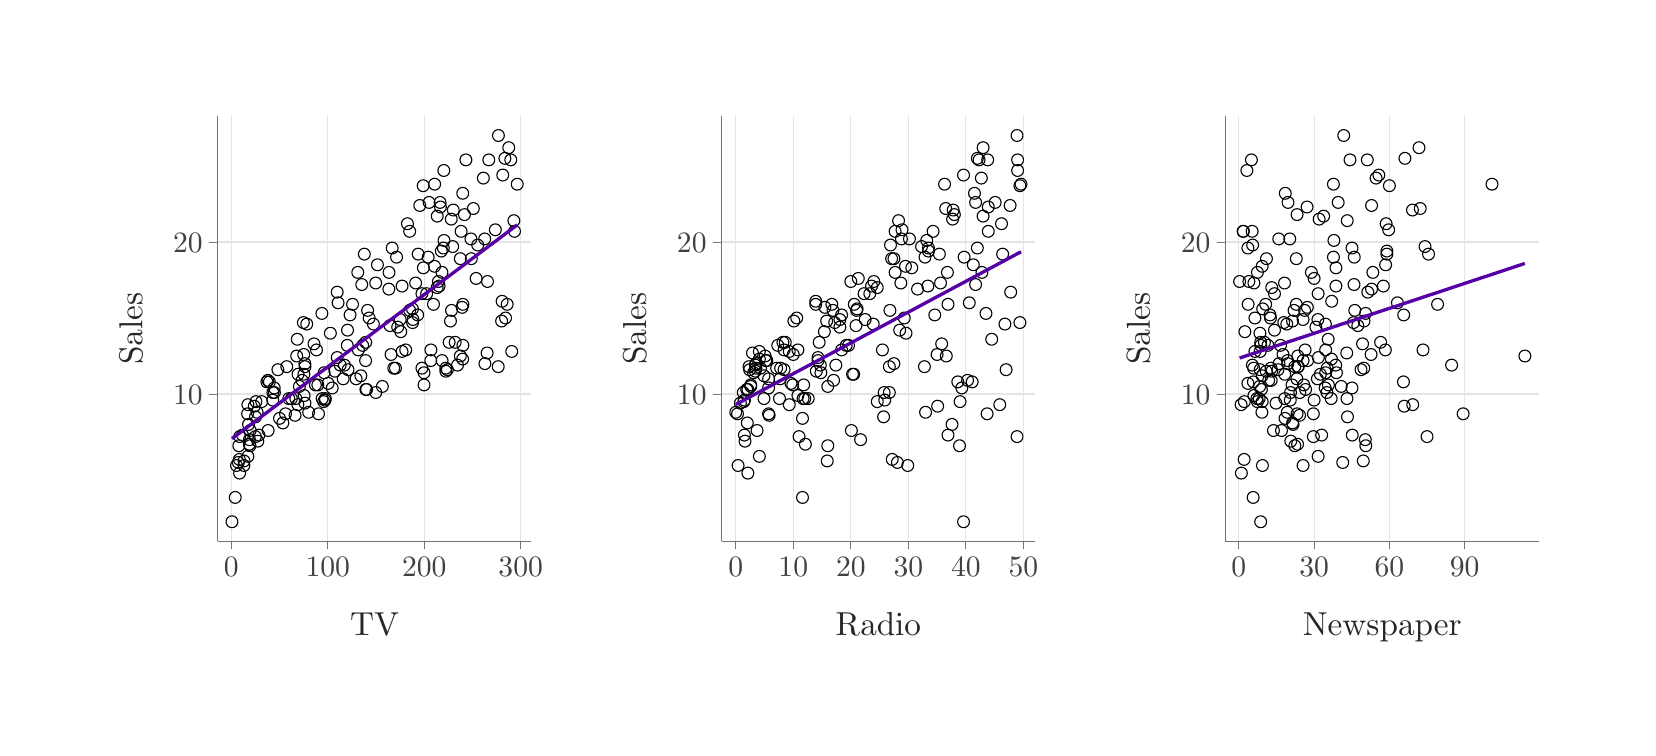
\begin{tikzpicture}[x=1pt,y=1pt]
\definecolor{fillColor}{RGB}{255,255,255}
\path[use as bounding box,fill=fillColor] (0,0) rectangle (578.16,252.94);
\begin{scope}
\path[clip] (  0.00,  0.00) rectangle (578.16,252.94);
\definecolor{drawColor}{RGB}{255,255,255}

\path[draw=drawColor,line width= 0.7pt,line join=round,line cap=round,fill=fillColor] ( -0.00,  0.00) rectangle (578.16,252.95);
\end{scope}
\begin{scope}
\path[clip] ( 16.00, 16.00) rectangle (198.05,236.95);
\definecolor{drawColor}{RGB}{255,255,255}
\definecolor{fillColor}{RGB}{255,255,255}

\path[draw=drawColor,line width= 0.6pt,line join=round,line cap=round,fill=fillColor] ( 16.00, 16.00) rectangle (198.05,236.95);
\end{scope}
\begin{scope}
\path[clip] (198.05, 16.00) rectangle (380.11,236.95);
\definecolor{drawColor}{RGB}{255,255,255}
\definecolor{fillColor}{RGB}{255,255,255}

\path[draw=drawColor,line width= 0.6pt,line join=round,line cap=round,fill=fillColor] (198.05, 16.00) rectangle (380.11,236.95);
\end{scope}
\begin{scope}
\path[clip] (380.11, 16.00) rectangle (562.16,236.95);
\definecolor{drawColor}{RGB}{255,255,255}
\definecolor{fillColor}{RGB}{255,255,255}

\path[draw=drawColor,line width= 0.6pt,line join=round,line cap=round,fill=fillColor] (380.11, 16.00) rectangle (562.16,236.95);
\end{scope}
\begin{scope}
\path[clip] ( 68.66, 67.42) rectangle (182.05,220.95);
\definecolor{drawColor}{RGB}{255,255,255}
\definecolor{fillColor}{RGB}{255,255,255}

\path[draw=drawColor,line width= 0.6pt,line join=round,line cap=round,fill=fillColor] ( 68.66, 67.42) rectangle (182.05,220.95);
\definecolor{drawColor}{RGB}{228,228,231}

\path[draw=drawColor,line width= 0.4pt,line join=round] ( 68.66,120.55) --
	(182.05,120.55);

\path[draw=drawColor,line width= 0.4pt,line join=round] ( 68.66,175.50) --
	(182.05,175.50);

\path[draw=drawColor,line width= 0.4pt,line join=round] ( 73.57, 67.42) --
	( 73.57,220.95);

\path[draw=drawColor,line width= 0.4pt,line join=round] (108.43, 67.42) --
	(108.43,220.95);

\path[draw=drawColor,line width= 0.4pt,line join=round] (143.29, 67.42) --
	(143.29,220.95);

\path[draw=drawColor,line width= 0.4pt,line join=round] (178.15, 67.42) --
	(178.15,220.95);
\definecolor{drawColor}{RGB}{0,0,0}

\path[draw=drawColor,line width= 0.4pt,line join=round,line cap=round] (153.79,187.04) circle (  2.14);

\path[draw=drawColor,line width= 0.4pt,line join=round,line cap=round] ( 89.09,122.75) circle (  2.14);

\path[draw=drawColor,line width= 0.4pt,line join=round,line cap=round] ( 79.57,116.71) circle (  2.14);

\path[draw=drawColor,line width= 0.4pt,line join=round,line cap=round] (126.39,167.26) circle (  2.14);

\path[draw=drawColor,line width= 0.4pt,line join=round,line cap=round] (136.60,136.49) circle (  2.14);

\path[draw=drawColor,line width= 0.4pt,line join=round,line cap=round] ( 76.61,105.17) circle (  2.14);

\path[draw=drawColor,line width= 0.4pt,line join=round,line cap=round] ( 93.62,130.45) circle (  2.14);

\path[draw=drawColor,line width= 0.4pt,line join=round,line cap=round] (115.48,138.14) circle (  2.14);

\path[draw=drawColor,line width= 0.4pt,line join=round,line cap=round] ( 76.57, 91.98) circle (  2.14);

\path[draw=drawColor,line width= 0.4pt,line join=round,line cap=round] (143.22,123.85) circle (  2.14);

\path[draw=drawColor,line width= 0.4pt,line join=round,line cap=round] ( 96.62,112.86) circle (  2.14);

\path[draw=drawColor,line width= 0.4pt,line join=round,line cap=round] (148.42,161.22) circle (  2.14);

\path[draw=drawColor,line width= 0.4pt,line join=round,line cap=round] ( 81.87,116.16) circle (  2.14);

\path[draw=drawColor,line width= 0.4pt,line join=round,line cap=round] (107.56,118.91) circle (  2.14);

\path[draw=drawColor,line width= 0.4pt,line join=round,line cap=round] (144.72,170.01) circle (  2.14);

\path[draw=drawColor,line width= 0.4pt,line join=round,line cap=round] (141.69,188.69) circle (  2.14);

\path[draw=drawColor,line width= 0.4pt,line join=round,line cap=round] ( 97.21,134.29) circle (  2.14);

\path[draw=drawColor,line width= 0.4pt,line join=round,line cap=round] (171.67,199.68) circle (  2.14);

\path[draw=drawColor,line width= 0.4pt,line join=round,line cap=round] ( 97.70,127.70) circle (  2.14);

\path[draw=drawColor,line width= 0.4pt,line join=round,line cap=round] (124.92,145.83) circle (  2.14);

\path[draw=drawColor,line width= 0.4pt,line join=round,line cap=round] (149.71,164.51) circle (  2.14);

\path[draw=drawColor,line width= 0.4pt,line join=round,line cap=round] (156.33,134.29) circle (  2.14);

\path[draw=drawColor,line width= 0.4pt,line join=round,line cap=round] ( 78.18, 96.38) circle (  2.14);

\path[draw=drawColor,line width= 0.4pt,line join=round,line cap=round] (153.16,150.78) circle (  2.14);

\path[draw=drawColor,line width= 0.4pt,line join=round,line cap=round] ( 95.29,118.91) circle (  2.14);

\path[draw=drawColor,line width= 0.4pt,line join=round,line cap=round] (165.22,131.54) circle (  2.14);

\path[draw=drawColor,line width= 0.4pt,line join=round,line cap=round] (123.39,148.03) circle (  2.14);

\path[draw=drawColor,line width= 0.4pt,line join=round,line cap=round] (157.27,152.97) circle (  2.14);

\path[draw=drawColor,line width= 0.4pt,line join=round,line cap=round] (160.31,169.46) circle (  2.14);

\path[draw=drawColor,line width= 0.4pt,line join=round,line cap=round] ( 98.19,123.30) circle (  2.14);

\path[draw=drawColor,line width= 0.4pt,line join=round,line cap=round] (175.68,183.20) circle (  2.14);

\path[draw=drawColor,line width= 0.4pt,line join=round,line cap=round] (112.93,131.00) circle (  2.14);

\path[draw=drawColor,line width= 0.4pt,line join=round,line cap=round] (107.46,118.36) circle (  2.14);

\path[draw=drawColor,line width= 0.4pt,line join=round,line cap=round] (166.16,161.22) circle (  2.14);

\path[draw=drawColor,line width= 0.4pt,line join=round,line cap=round] (106.94,117.81) circle (  2.14);

\path[draw=drawColor,line width= 0.4pt,line join=round,line cap=round] (174.91,135.94) circle (  2.14);

\path[draw=drawColor,line width= 0.4pt,line join=round,line cap=round] (166.62,205.17) circle (  2.14);

\path[draw=drawColor,line width= 0.4pt,line join=round,line cap=round] ( 99.62,146.38) circle (  2.14);

\path[draw=drawColor,line width= 0.4pt,line join=round,line cap=round] ( 88.60,121.10) circle (  2.14);

\path[draw=drawColor,line width= 0.4pt,line join=round,line cap=round] (153.06,183.75) circle (  2.14);

\path[draw=drawColor,line width= 0.4pt,line join=round,line cap=round] (144.17,156.82) circle (  2.14);

\path[draw=drawColor,line width= 0.4pt,line join=round,line cap=round] (135.28,159.57) circle (  2.14);

\path[draw=drawColor,line width= 0.4pt,line join=round,line cap=round] (175.92,179.35) circle (  2.14);

\path[draw=drawColor,line width= 0.4pt,line join=round,line cap=round] (145.70,136.49) circle (  2.14);

\path[draw=drawColor,line width= 0.4pt,line join=round,line cap=round] ( 82.32,112.31) circle (  2.14);

\path[draw=drawColor,line width= 0.4pt,line join=round,line cap=round] (134.61,147.48) circle (  2.14);

\path[draw=drawColor,line width= 0.4pt,line join=round,line cap=round] (104.84,123.85) circle (  2.14);

\path[draw=drawColor,line width= 0.4pt,line join=round,line cap=round] (157.20,193.09) circle (  2.14);

\path[draw=drawColor,line width= 0.4pt,line join=round,line cap=round] (152.78,146.93) circle (  2.14);

\path[draw=drawColor,line width= 0.4pt,line join=round,line cap=round] ( 96.90,118.91) circle (  2.14);

\path[draw=drawColor,line width= 0.4pt,line join=round,line cap=round] (143.22,128.25) circle (  2.14);

\path[draw=drawColor,line width= 0.4pt,line join=round,line cap=round] (108.57,124.40) circle (  2.14);

\path[draw=drawColor,line width= 0.4pt,line join=round,line cap=round] (149.01,189.79) circle (  2.14);

\path[draw=drawColor,line width= 0.4pt,line join=round,line cap=round] (137.23,182.10) circle (  2.14);

\path[draw=drawColor,line width= 0.4pt,line join=round,line cap=round] (165.15,176.60) circle (  2.14);

\path[draw=drawColor,line width= 0.4pt,line join=round,line cap=round] (142.91,195.83) circle (  2.14);

\path[draw=drawColor,line width= 0.4pt,line join=round,line cap=round] ( 76.12, 95.83) circle (  2.14);

\path[draw=drawColor,line width= 0.4pt,line join=round,line cap=round] (121.05,138.14) circle (  2.14);

\path[draw=drawColor,line width= 0.4pt,line join=round,line cap=round] (147.06,196.38) circle (  2.14);

\path[draw=drawColor,line width= 0.4pt,line join=round,line cap=round] (147.02,166.71) circle (  2.14);

\path[draw=drawColor,line width= 0.4pt,line join=round,line cap=round] ( 92.22,110.11) circle (  2.14);

\path[draw=drawColor,line width= 0.4pt,line join=round,line cap=round] (164.66,198.58) circle (  2.14);

\path[draw=drawColor,line width= 0.4pt,line join=round,line cap=round] (156.99,151.88) circle (  2.14);

\path[draw=drawColor,line width= 0.4pt,line join=round,line cap=round] (109.38,142.53) circle (  2.14);

\path[draw=drawColor,line width= 0.4pt,line join=round,line cap=round] (119.28,164.51) circle (  2.14);

\path[draw=drawColor,line width= 0.4pt,line join=round,line cap=round] ( 97.63,116.71) circle (  2.14);

\path[draw=drawColor,line width= 0.4pt,line join=round,line cap=round] ( 84.56,117.81) circle (  2.14);

\path[draw=drawColor,line width= 0.4pt,line join=round,line cap=round] (122.13,139.24) circle (  2.14);

\path[draw=drawColor,line width= 0.4pt,line join=round,line cap=round] (156.33,169.46) circle (  2.14);

\path[draw=drawColor,line width= 0.4pt,line join=round,line cap=round] (149.15,188.14) circle (  2.14);

\path[draw=drawColor,line width= 0.4pt,line join=round,line cap=round] (142.98,166.16) circle (  2.14);

\path[draw=drawColor,line width= 0.4pt,line join=round,line cap=round] (111.85,133.74) circle (  2.14);

\path[draw=drawColor,line width= 0.4pt,line join=round,line cap=round] ( 82.92,113.96) circle (  2.14);

\path[draw=drawColor,line width= 0.4pt,line join=round,line cap=round] (118.68,126.05) circle (  2.14);

\path[draw=drawColor,line width= 0.4pt,line join=round,line cap=round] (147.97,159.02) circle (  2.14);

\path[draw=drawColor,line width= 0.4pt,line join=round,line cap=round] ( 79.47,113.41) circle (  2.14);

\path[draw=drawColor,line width= 0.4pt,line join=round,line cap=round] ( 83.16,103.52) circle (  2.14);

\path[draw=drawColor,line width= 0.4pt,line join=round,line cap=round] (115.58,143.63) circle (  2.14);

\path[draw=drawColor,line width= 0.4pt,line join=round,line cap=round] ( 75.46, 94.73) circle (  2.14);

\path[draw=drawColor,line width= 0.4pt,line join=round,line cap=round] (114.01,126.05) circle (  2.14);

\path[draw=drawColor,line width= 0.4pt,line join=round,line cap=round] (100.21,130.45) circle (  2.14);

\path[draw=drawColor,line width= 0.4pt,line join=round,line cap=round] (157.17,133.19) circle (  2.14);

\path[draw=drawColor,line width= 0.4pt,line join=round,line cap=round] ( 99.82,127.70) circle (  2.14);

\path[draw=drawColor,line width= 0.4pt,line join=round,line cap=round] ( 97.42,140.34) circle (  2.14);

\path[draw=drawColor,line width= 0.4pt,line join=round,line cap=round] (148.00,184.84) circle (  2.14);

\path[draw=drawColor,line width= 0.4pt,line join=round,line cap=round] (140.92,149.13) circle (  2.14);

\path[draw=drawColor,line width= 0.4pt,line join=round,line cap=round] (100.17,131.54) circle (  2.14);

\path[draw=drawColor,line width= 0.4pt,line join=round,line cap=round] (112.16,153.52) circle (  2.14);

\path[draw=drawColor,line width= 0.4pt,line join=round,line cap=round] (104.36,136.49) circle (  2.14);

\path[draw=drawColor,line width= 0.4pt,line join=round,line cap=round] (111.85,157.37) circle (  2.14);

\path[draw=drawColor,line width= 0.4pt,line join=round,line cap=round] (120.39,127.15) circle (  2.14);

\path[draw=drawColor,line width= 0.4pt,line join=round,line cap=round] ( 83.54,105.72) circle (  2.14);

\path[draw=drawColor,line width= 0.4pt,line join=round,line cap=round] (149.46,172.21) circle (  2.14);

\path[draw=drawColor,line width= 0.4pt,line join=round,line cap=round] (161.04,187.59) circle (  2.14);

\path[draw=drawColor,line width= 0.4pt,line join=round,line cap=round] (111.01,128.80) circle (  2.14);

\path[draw=drawColor,line width= 0.4pt,line join=round,line cap=round] (130.50,158.47) circle (  2.14);

\path[draw=drawColor,line width= 0.4pt,line join=round,line cap=round] (142.46,129.90) circle (  2.14);

\path[draw=drawColor,line width= 0.4pt,line join=round,line cap=round] (138.03,150.78) circle (  2.14);

\path[draw=drawColor,line width= 0.4pt,line join=round,line cap=round] (174.56,205.17) circle (  2.14);

\path[draw=drawColor,line width= 0.4pt,line join=round,line cap=round] (120.71,160.12) circle (  2.14);

\path[draw=drawColor,line width= 0.4pt,line join=round,line cap=round] (151.10,129.90) circle (  2.14);

\path[draw=drawColor,line width= 0.4pt,line join=round,line cap=round] (176.90,196.38) circle (  2.14);

\path[draw=drawColor,line width= 0.4pt,line join=round,line cap=round] (171.25,146.93) circle (  2.14);

\path[draw=drawColor,line width= 0.4pt,line join=round,line cap=round] (139.08,146.38) circle (  2.14);

\path[draw=drawColor,line width= 0.4pt,line join=round,line cap=round] (156.61,179.35) circle (  2.14);

\path[draw=drawColor,line width= 0.4pt,line join=round,line cap=round] (121.65,171.11) circle (  2.14);

\path[draw=drawColor,line width= 0.4pt,line join=round,line cap=round] ( 82.29,105.17) circle (  2.14);

\path[draw=drawColor,line width= 0.4pt,line join=round,line cap=round] (105.09,113.41) circle (  2.14);

\path[draw=drawColor,line width= 0.4pt,line join=round,line cap=round] ( 78.14, 94.73) circle (  2.14);

\path[draw=drawColor,line width= 0.4pt,line join=round,line cap=round] (162.61,174.40) circle (  2.14);

\path[draw=drawColor,line width= 0.4pt,line join=round,line cap=round] (152.29,139.24) circle (  2.14);

\path[draw=drawColor,line width= 0.4pt,line join=round,line cap=round] (157.83,185.39) circle (  2.14);

\path[draw=drawColor,line width= 0.4pt,line join=round,line cap=round] (134.82,143.08) circle (  2.14);

\path[draw=drawColor,line width= 0.4pt,line join=round,line cap=round] (146.64,152.97) circle (  2.14);

\path[draw=drawColor,line width= 0.4pt,line join=round,line cap=round] (100.84,145.83) circle (  2.14);

\path[draw=drawColor,line width= 0.4pt,line join=round,line cap=round] ( 99.75,134.84) circle (  2.14);

\path[draw=drawColor,line width= 0.4pt,line join=round,line cap=round] (122.10,132.64) circle (  2.14);

\path[draw=drawColor,line width= 0.4pt,line join=round,line cap=round] (100.21,117.26) circle (  2.14);

\path[draw=drawColor,line width= 0.4pt,line join=round,line cap=round] (117.39,152.97) circle (  2.14);

\path[draw=drawColor,line width= 0.4pt,line join=round,line cap=round] ( 80.34,101.87) circle (  2.14);

\path[draw=drawColor,line width= 0.4pt,line join=round,line cap=round] (122.83,150.78) circle (  2.14);

\path[draw=drawColor,line width= 0.4pt,line join=round,line cap=round] ( 80.13,104.07) circle (  2.14);

\path[draw=drawColor,line width= 0.4pt,line join=round,line cap=round] (151.66,129.35) circle (  2.14);

\path[draw=drawColor,line width= 0.4pt,line join=round,line cap=round] (116.49,149.13) circle (  2.14);

\path[draw=drawColor,line width= 0.4pt,line join=round,line cap=round] (153.58,173.85) circle (  2.14);

\path[draw=drawColor,line width= 0.4pt,line join=round,line cap=round] (103.97,123.85) circle (  2.14);

\path[draw=drawColor,line width= 0.4pt,line join=round,line cap=round] ( 76.29,101.87) circle (  2.14);

\path[draw=drawColor,line width= 0.4pt,line join=round,line cap=round] (101.53,113.96) circle (  2.14);

\path[draw=drawColor,line width= 0.4pt,line join=round,line cap=round] (150.37,201.33) circle (  2.14);

\path[draw=drawColor,line width= 0.4pt,line join=round,line cap=round] ( 94.35,118.91) circle (  2.14);

\path[draw=drawColor,line width= 0.4pt,line join=round,line cap=round] ( 73.82, 74.40) circle (  2.14);

\path[draw=drawColor,line width= 0.4pt,line join=round,line cap=round] (166.02,135.39) circle (  2.14);

\path[draw=drawColor,line width= 0.4pt,line join=round,line cap=round] ( 76.50, 96.93) circle (  2.14);

\path[draw=drawColor,line width= 0.4pt,line join=round,line cap=round] (150.20,173.31) circle (  2.14);

\path[draw=drawColor,line width= 0.4pt,line join=round,line cap=round] ( 86.44,124.95) circle (  2.14);

\path[draw=drawColor,line width= 0.4pt,line join=round,line cap=round] ( 90.41,129.35) circle (  2.14);

\path[draw=drawColor,line width= 0.4pt,line join=round,line cap=round] ( 82.50,117.81) circle (  2.14);

\path[draw=drawColor,line width= 0.4pt,line join=round,line cap=round] (168.99,179.90) circle (  2.14);

\path[draw=drawColor,line width= 0.4pt,line join=round,line cap=round] ( 88.56,118.36) circle (  2.14);

\path[draw=drawColor,line width= 0.4pt,line join=round,line cap=round] (138.03,179.35) circle (  2.14);

\path[draw=drawColor,line width= 0.4pt,line join=round,line cap=round] ( 99.16,125.50) circle (  2.14);

\path[draw=drawColor,line width= 0.4pt,line join=round,line cap=round] (141.10,171.11) circle (  2.14);

\path[draw=drawColor,line width= 0.4pt,line join=round,line cap=round] (150.44,176.05) circle (  2.14);

\path[draw=drawColor,line width= 0.4pt,line join=round,line cap=round] (110.04,122.75) circle (  2.14);

\path[draw=drawColor,line width= 0.4pt,line join=round,line cap=round] (107.11,128.25) circle (  2.14);

\path[draw=drawColor,line width= 0.4pt,line join=round,line cap=round] (122.48,122.20) circle (  2.14);

\path[draw=drawColor,line width= 0.4pt,line join=round,line cap=round] (157.27,138.14) circle (  2.14);

\path[draw=drawColor,line width= 0.4pt,line join=round,line cap=round] (158.35,205.17) circle (  2.14);

\path[draw=drawColor,line width= 0.4pt,line join=round,line cap=round] ( 86.82,125.50) circle (  2.14);

\path[draw=drawColor,line width= 0.4pt,line join=round,line cap=round] ( 89.16,121.10) circle (  2.14);

\path[draw=drawColor,line width= 0.4pt,line join=round,line cap=round] (171.43,154.07) circle (  2.14);

\path[draw=drawColor,line width= 0.4pt,line join=round,line cap=round] (115.76,129.35) circle (  2.14);

\path[draw=drawColor,line width= 0.4pt,line join=round,line cap=round] (142.46,156.82) circle (  2.14);

\path[draw=drawColor,line width= 0.4pt,line join=round,line cap=round] (133.29,170.01) circle (  2.14);

\path[draw=drawColor,line width= 0.4pt,line join=round,line cap=round] (139.04,151.33) circle (  2.14);

\path[draw=drawColor,line width= 0.4pt,line join=round,line cap=round] ( 75.00, 83.19) circle (  2.14);

\path[draw=drawColor,line width= 0.4pt,line join=round,line cap=round] (106.31,149.68) circle (  2.14);

\path[draw=drawColor,line width= 0.4pt,line join=round,line cap=round] (125.79,121.10) circle (  2.14);

\path[draw=drawColor,line width= 0.4pt,line join=round,line cap=round] ( 77.65,105.72) circle (  2.14);

\path[draw=drawColor,line width= 0.4pt,line join=round,line cap=round] (119.49,136.49) circle (  2.14);

\path[draw=drawColor,line width= 0.4pt,line join=round,line cap=round] (133.71,144.73) circle (  2.14);

\path[draw=drawColor,line width= 0.4pt,line join=round,line cap=round] (103.45,138.69) circle (  2.14);

\path[draw=drawColor,line width= 0.4pt,line join=round,line cap=round] (139.25,147.48) circle (  2.14);

\path[draw=drawColor,line width= 0.4pt,line join=round,line cap=round] (130.57,164.51) circle (  2.14);

\path[draw=drawColor,line width= 0.4pt,line join=round,line cap=round] (114.43,131.00) circle (  2.14);

\path[draw=drawColor,line width= 0.4pt,line join=round,line cap=round] (155.32,131.00) circle (  2.14);

\path[draw=drawColor,line width= 0.4pt,line join=round,line cap=round] ( 79.81,109.57) circle (  2.14);

\path[draw=drawColor,line width= 0.4pt,line join=round,line cap=round] (145.66,132.64) circle (  2.14);

\path[draw=drawColor,line width= 0.4pt,line join=round,line cap=round] (148.66,159.57) circle (  2.14);

\path[draw=drawColor,line width= 0.4pt,line join=round,line cap=round] (172.68,148.03) circle (  2.14);

\path[draw=drawColor,line width= 0.4pt,line join=round,line cap=round] ( 91.00,111.76) circle (  2.14);

\path[draw=drawColor,line width= 0.4pt,line join=round,line cap=round] (130.92,145.28) circle (  2.14);

\path[draw=drawColor,line width= 0.4pt,line join=round,line cap=round] ( 80.41,107.37) circle (  2.14);

\path[draw=drawColor,line width= 0.4pt,line join=round,line cap=round] (132.28,129.90) circle (  2.14);

\path[draw=drawColor,line width= 0.4pt,line join=round,line cap=round] (151.10,128.80) circle (  2.14);

\path[draw=drawColor,line width= 0.4pt,line join=round,line cap=round] (170.10,213.97) circle (  2.14);

\path[draw=drawColor,line width= 0.4pt,line join=round,line cap=round] (160.17,176.60) circle (  2.14);

\path[draw=drawColor,line width= 0.4pt,line join=round,line cap=round] (132.91,129.90) circle (  2.14);

\path[draw=drawColor,line width= 0.4pt,line join=round,line cap=round] (170.03,130.45) circle (  2.14);

\path[draw=drawColor,line width= 0.4pt,line join=round,line cap=round] (131.30,134.84) circle (  2.14);

\path[draw=drawColor,line width= 0.4pt,line join=round,line cap=round] (128.17,123.30) circle (  2.14);

\path[draw=drawColor,line width= 0.4pt,line join=round,line cap=round] (149.74,132.64) circle (  2.14);

\path[draw=drawColor,line width= 0.4pt,line join=round,line cap=round] ( 93.17,113.41) circle (  2.14);

\path[draw=drawColor,line width= 0.4pt,line join=round,line cap=round] (173.83,209.57) circle (  2.14);

\path[draw=drawColor,line width= 0.4pt,line join=round,line cap=round] (162.05,162.32) circle (  2.14);

\path[draw=drawColor,line width= 0.4pt,line join=round,line cap=round] (145.04,189.79) circle (  2.14);

\path[draw=drawColor,line width= 0.4pt,line join=round,line cap=round] (122.20,122.20) circle (  2.14);

\path[draw=drawColor,line width= 0.4pt,line join=round,line cap=round] (140.19,160.67) circle (  2.14);

\path[draw=drawColor,line width= 0.4pt,line join=round,line cap=round] (173.27,152.97) circle (  2.14);

\path[draw=drawColor,line width= 0.4pt,line join=round,line cap=round] ( 80.09,102.42) circle (  2.14);

\path[draw=drawColor,line width= 0.4pt,line join=round,line cap=round] ( 87.34,124.95) circle (  2.14);

\path[draw=drawColor,line width= 0.4pt,line join=round,line cap=round] ( 99.89,120.01) circle (  2.14);

\path[draw=drawColor,line width= 0.4pt,line join=round,line cap=round] ( 79.57, 98.03) circle (  2.14);

\path[draw=drawColor,line width= 0.4pt,line join=round,line cap=round] (131.72,173.31) circle (  2.14);

\path[draw=drawColor,line width= 0.4pt,line join=round,line cap=round] (125.76,160.67) circle (  2.14);

\path[draw=drawColor,line width= 0.4pt,line join=round,line cap=round] ( 86.89,107.37) circle (  2.14);

\path[draw=drawColor,line width= 0.4pt,line join=round,line cap=round] (106.41,118.91) circle (  2.14);

\path[draw=drawColor,line width= 0.4pt,line join=round,line cap=round] (135.28,135.94) circle (  2.14);

\path[draw=drawColor,line width= 0.4pt,line join=round,line cap=round] (172.44,205.72) circle (  2.14);

\path[draw=drawColor,line width= 0.4pt,line join=round,line cap=round] (154.48,139.24) circle (  2.14);
\definecolor{drawColor}{RGB}{86,1,165}

\path[draw=drawColor,line width= 1.2pt,line join=round] ( 73.82,104.43) --
	( 75.12,105.41) --
	( 76.43,106.39) --
	( 77.73,107.37) --
	( 79.04,108.34) --
	( 80.34,109.32) --
	( 81.65,110.30) --
	( 82.95,111.28) --
	( 84.26,112.25) --
	( 85.56,113.23) --
	( 86.87,114.21) --
	( 88.17,115.19) --
	( 89.48,116.16) --
	( 90.78,117.14) --
	( 92.09,118.12) --
	( 93.39,119.10) --
	( 94.70,120.08) --
	( 96.00,121.05) --
	( 97.31,122.03) --
	( 98.61,123.01) --
	( 99.92,123.99) --
	(101.22,124.96) --
	(102.52,125.94) --
	(103.83,126.92) --
	(105.13,127.90) --
	(106.44,128.87) --
	(107.74,129.85) --
	(109.05,130.83) --
	(110.35,131.81) --
	(111.66,132.79) --
	(112.96,133.76) --
	(114.27,134.74) --
	(115.57,135.72) --
	(116.88,136.70) --
	(118.18,137.67) --
	(119.49,138.65) --
	(120.79,139.63) --
	(122.10,140.61) --
	(123.40,141.59) --
	(124.71,142.56) --
	(126.01,143.54) --
	(127.32,144.52) --
	(128.62,145.50) --
	(129.93,146.47) --
	(131.23,147.45) --
	(132.54,148.43) --
	(133.84,149.41) --
	(135.15,150.38) --
	(136.45,151.36) --
	(137.75,152.34) --
	(139.06,153.32) --
	(140.36,154.30) --
	(141.67,155.27) --
	(142.97,156.25) --
	(144.28,157.23) --
	(145.58,158.21) --
	(146.89,159.18) --
	(148.19,160.16) --
	(149.50,161.14) --
	(150.80,162.12) --
	(152.11,163.09) --
	(153.41,164.07) --
	(154.72,165.05) --
	(156.02,166.03) --
	(157.33,167.01) --
	(158.63,167.98) --
	(159.94,168.96) --
	(161.24,169.94) --
	(162.55,170.92) --
	(163.85,171.89) --
	(165.16,172.87) --
	(166.46,173.85) --
	(167.77,174.83) --
	(169.07,175.80) --
	(170.38,176.78) --
	(171.68,177.76) --
	(172.98,178.74) --
	(174.29,179.72) --
	(175.59,180.69) --
	(176.90,181.67);
\end{scope}
\begin{scope}
\path[clip] (  0.00,  0.00) rectangle (578.16,252.94);
\definecolor{drawColor}{RGB}{113,113,122}

\path[draw=drawColor,line width= 0.3pt,line join=round] ( 68.66, 67.42) --
	( 68.66,220.95);
\end{scope}
\begin{scope}
\path[clip] (  0.00,  0.00) rectangle (578.16,252.94);
\definecolor{drawColor}{RGB}{63,63,70}

\node[text=drawColor,anchor=base east,inner sep=0pt, outer sep=0pt, scale=  1.07] at ( 63.26,116.88) {10};

\node[text=drawColor,anchor=base east,inner sep=0pt, outer sep=0pt, scale=  1.07] at ( 63.26,171.83) {20};
\end{scope}
\begin{scope}
\path[clip] (  0.00,  0.00) rectangle (578.16,252.94);
\definecolor{drawColor}{RGB}{113,113,122}

\path[draw=drawColor,line width= 0.3pt,line join=round] ( 65.66,120.55) --
	( 68.66,120.55);

\path[draw=drawColor,line width= 0.3pt,line join=round] ( 65.66,175.50) --
	( 68.66,175.50);
\end{scope}
\begin{scope}
\path[clip] (  0.00,  0.00) rectangle (578.16,252.94);
\definecolor{drawColor}{RGB}{113,113,122}

\path[draw=drawColor,line width= 0.3pt,line join=round] ( 68.66, 67.42) --
	(182.05, 67.42);
\end{scope}
\begin{scope}
\path[clip] (  0.00,  0.00) rectangle (578.16,252.94);
\definecolor{drawColor}{RGB}{113,113,122}

\path[draw=drawColor,line width= 0.3pt,line join=round] ( 73.57, 64.42) --
	( 73.57, 67.42);

\path[draw=drawColor,line width= 0.3pt,line join=round] (108.43, 64.42) --
	(108.43, 67.42);

\path[draw=drawColor,line width= 0.3pt,line join=round] (143.29, 64.42) --
	(143.29, 67.42);

\path[draw=drawColor,line width= 0.3pt,line join=round] (178.15, 64.42) --
	(178.15, 67.42);
\end{scope}
\begin{scope}
\path[clip] (  0.00,  0.00) rectangle (578.16,252.94);
\definecolor{drawColor}{RGB}{63,63,70}

\node[text=drawColor,anchor=base,inner sep=0pt, outer sep=0pt, scale=  1.07] at ( 73.57, 54.67) {0};

\node[text=drawColor,anchor=base,inner sep=0pt, outer sep=0pt, scale=  1.07] at (108.43, 54.67) {100};

\node[text=drawColor,anchor=base,inner sep=0pt, outer sep=0pt, scale=  1.07] at (143.29, 54.67) {200};

\node[text=drawColor,anchor=base,inner sep=0pt, outer sep=0pt, scale=  1.07] at (178.15, 54.67) {300};
\end{scope}
\begin{scope}
\path[clip] (  0.00,  0.00) rectangle (578.16,252.94);
\definecolor{drawColor}{RGB}{39,39,42}

\node[text=drawColor,anchor=base,inner sep=0pt, outer sep=0pt, scale=  1.20] at (125.36, 33.17) {TV};
\end{scope}
\begin{scope}
\path[clip] (  0.00,  0.00) rectangle (578.16,252.94);
\definecolor{drawColor}{RGB}{39,39,42}

\node[text=drawColor,rotate= 90.00,anchor=base,inner sep=0pt, outer sep=0pt, scale=  1.20] at ( 41.43,144.18) {Sales};
\end{scope}
\begin{scope}
\path[clip] (250.72, 67.42) rectangle (364.11,220.95);
\definecolor{drawColor}{RGB}{255,255,255}
\definecolor{fillColor}{RGB}{255,255,255}

\path[draw=drawColor,line width= 0.6pt,line join=round,line cap=round,fill=fillColor] (250.72, 67.42) rectangle (364.11,220.95);
\definecolor{drawColor}{RGB}{228,228,231}

\path[draw=drawColor,line width= 0.4pt,line join=round] (250.72,120.55) --
	(364.11,120.55);

\path[draw=drawColor,line width= 0.4pt,line join=round] (250.72,175.50) --
	(364.11,175.50);

\path[draw=drawColor,line width= 0.4pt,line join=round] (255.87, 67.42) --
	(255.87,220.95);

\path[draw=drawColor,line width= 0.4pt,line join=round] (276.65, 67.42) --
	(276.65,220.95);

\path[draw=drawColor,line width= 0.4pt,line join=round] (297.44, 67.42) --
	(297.44,220.95);

\path[draw=drawColor,line width= 0.4pt,line join=round] (318.22, 67.42) --
	(318.22,220.95);

\path[draw=drawColor,line width= 0.4pt,line join=round] (339.00, 67.42) --
	(339.00,220.95);

\path[draw=drawColor,line width= 0.4pt,line join=round] (359.78, 67.42) --
	(359.78,220.95);
\definecolor{drawColor}{RGB}{0,0,0}

\path[draw=drawColor,line width= 0.4pt,line join=round,line cap=round] (334.43,187.04) circle (  2.14);

\path[draw=drawColor,line width= 0.4pt,line join=round,line cap=round] (337.55,122.75) circle (  2.14);

\path[draw=drawColor,line width= 0.4pt,line join=round,line cap=round] (351.26,116.71) circle (  2.14);

\path[draw=drawColor,line width= 0.4pt,line join=round,line cap=round] (341.70,167.26) circle (  2.14);

\path[draw=drawColor,line width= 0.4pt,line join=round,line cap=round] (278.32,136.49) circle (  2.14);

\path[draw=drawColor,line width= 0.4pt,line join=round,line cap=round] (357.50,105.17) circle (  2.14);

\path[draw=drawColor,line width= 0.4pt,line join=round,line cap=round] (324.04,130.45) circle (  2.14);

\path[draw=drawColor,line width= 0.4pt,line join=round,line cap=round] (296.61,138.14) circle (  2.14);

\path[draw=drawColor,line width= 0.4pt,line join=round,line cap=round] (260.24, 91.98) circle (  2.14);

\path[draw=drawColor,line width= 0.4pt,line join=round,line cap=round] (261.28,123.85) circle (  2.14);

\path[draw=drawColor,line width= 0.4pt,line join=round,line cap=round] (267.93,112.86) circle (  2.14);

\path[draw=drawColor,line width= 0.4pt,line join=round,line cap=round] (305.75,161.22) circle (  2.14);

\path[draw=drawColor,line width= 0.4pt,line join=round,line cap=round] (328.82,116.16) circle (  2.14);

\path[draw=drawColor,line width= 0.4pt,line join=round,line cap=round] (271.67,118.91) circle (  2.14);

\path[draw=drawColor,line width= 0.4pt,line join=round,line cap=round] (324.25,170.01) circle (  2.14);

\path[draw=drawColor,line width= 0.4pt,line join=round,line cap=round] (355.00,188.69) circle (  2.14);

\path[draw=drawColor,line width= 0.4pt,line join=round,line cap=round] (331.94,134.29) circle (  2.14);

\path[draw=drawColor,line width= 0.4pt,line join=round,line cap=round] (338.17,199.68) circle (  2.14);

\path[draw=drawColor,line width= 0.4pt,line join=round,line cap=round] (298.48,127.70) circle (  2.14);

\path[draw=drawColor,line width= 0.4pt,line join=round,line cap=round] (305.54,145.83) circle (  2.14);

\path[draw=drawColor,line width= 0.4pt,line join=round,line cap=round] (313.44,164.51) circle (  2.14);

\path[draw=drawColor,line width= 0.4pt,line join=round,line cap=round] (266.47,134.29) circle (  2.14);

\path[draw=drawColor,line width= 0.4pt,line join=round,line cap=round] (288.92, 96.38) circle (  2.14);

\path[draw=drawColor,line width= 0.4pt,line join=round,line cap=round] (290.99,150.78) circle (  2.14);

\path[draw=drawColor,line width= 0.4pt,line join=round,line cap=round] (282.06,118.91) circle (  2.14);

\path[draw=drawColor,line width= 0.4pt,line join=round,line cap=round] (263.15,131.54) circle (  2.14);

\path[draw=drawColor,line width= 0.4pt,line join=round,line cap=round] (316.76,148.03) circle (  2.14);

\path[draw=drawColor,line width= 0.4pt,line join=round,line cap=round] (290.58,152.97) circle (  2.14);

\path[draw=drawColor,line width= 0.4pt,line join=round,line cap=round] (312.19,169.46) circle (  2.14);

\path[draw=drawColor,line width= 0.4pt,line join=round,line cap=round] (289.12,123.30) circle (  2.14);

\path[draw=drawColor,line width= 0.4pt,line join=round,line cap=round] (314.69,183.20) circle (  2.14);

\path[draw=drawColor,line width= 0.4pt,line join=round,line cap=round] (292.03,131.00) circle (  2.14);

\path[draw=drawColor,line width= 0.4pt,line join=round,line cap=round] (258.99,118.36) circle (  2.14);

\path[draw=drawColor,line width= 0.4pt,line join=round,line cap=round] (297.44,161.22) circle (  2.14);

\path[draw=drawColor,line width= 0.4pt,line join=round,line cap=round] (258.78,117.81) circle (  2.14);

\path[draw=drawColor,line width= 0.4pt,line join=round,line cap=round] (264.39,135.94) circle (  2.14);

\path[draw=drawColor,line width= 0.4pt,line join=round,line cap=round] (346.90,205.17) circle (  2.14);

\path[draw=drawColor,line width= 0.4pt,line join=round,line cap=round] (358.54,146.38) circle (  2.14);

\path[draw=drawColor,line width= 0.4pt,line join=round,line cap=round] (311.36,121.10) circle (  2.14);

\path[draw=drawColor,line width= 0.4pt,line join=round,line cap=round] (334.22,183.75) circle (  2.14);

\path[draw=drawColor,line width= 0.4pt,line join=round,line cap=round] (302.22,156.82) circle (  2.14);

\path[draw=drawColor,line width= 0.4pt,line join=round,line cap=round] (325.29,159.57) circle (  2.14);

\path[draw=drawColor,line width= 0.4pt,line join=round,line cap=round] (313.44,179.35) circle (  2.14);

\path[draw=drawColor,line width= 0.4pt,line join=round,line cap=round] (273.33,136.49) circle (  2.14);

\path[draw=drawColor,line width= 0.4pt,line join=round,line cap=round] (309.28,112.31) circle (  2.14);

\path[draw=drawColor,line width= 0.4pt,line join=round,line cap=round] (302.63,147.48) circle (  2.14);

\path[draw=drawColor,line width= 0.4pt,line join=round,line cap=round] (276.45,123.85) circle (  2.14);

\path[draw=drawColor,line width= 0.4pt,line join=round,line cap=round] (342.12,193.09) circle (  2.14);

\path[draw=drawColor,line width= 0.4pt,line join=round,line cap=round] (288.71,146.93) circle (  2.14);

\path[draw=drawColor,line width= 0.4pt,line join=round,line cap=round] (280.19,118.91) circle (  2.14);

\path[draw=drawColor,line width= 0.4pt,line join=round,line cap=round] (262.31,128.25) circle (  2.14);

\path[draw=drawColor,line width= 0.4pt,line join=round,line cap=round] (275.82,124.40) circle (  2.14);

\path[draw=drawColor,line width= 0.4pt,line join=round,line cap=round] (342.53,189.79) circle (  2.14);

\path[draw=drawColor,line width= 0.4pt,line join=round,line cap=round] (351.89,182.10) circle (  2.14);

\path[draw=drawColor,line width= 0.4pt,line join=round,line cap=round] (315.73,176.60) circle (  2.14);

\path[draw=drawColor,line width= 0.4pt,line join=round,line cap=round] (358.54,195.83) circle (  2.14);

\path[draw=drawColor,line width= 0.4pt,line join=round,line cap=round] (314.27, 95.83) circle (  2.14);

\path[draw=drawColor,line width= 0.4pt,line join=round,line cap=round] (295.77,138.14) circle (  2.14);

\path[draw=drawColor,line width= 0.4pt,line join=round,line cap=round] (358.95,196.38) circle (  2.14);

\path[draw=drawColor,line width= 0.4pt,line join=round,line cap=round] (317.18,166.71) circle (  2.14);

\path[draw=drawColor,line width= 0.4pt,line join=round,line cap=round] (260.03,110.11) circle (  2.14);

\path[draw=drawColor,line width= 0.4pt,line join=round,line cap=round] (344.61,198.58) circle (  2.14);

\path[draw=drawColor,line width= 0.4pt,line join=round,line cap=round] (288.08,151.88) circle (  2.14);

\path[draw=drawColor,line width= 0.4pt,line join=round,line cap=round] (317.39,142.53) circle (  2.14);

\path[draw=drawColor,line width= 0.4pt,line join=round,line cap=round] (344.82,164.51) circle (  2.14);

\path[draw=drawColor,line width= 0.4pt,line join=round,line cap=round] (275.20,116.71) circle (  2.14);

\path[draw=drawColor,line width= 0.4pt,line join=round,line cap=round] (307.00,117.81) circle (  2.14);

\path[draw=drawColor,line width= 0.4pt,line join=round,line cap=round] (286.01,139.24) circle (  2.14);

\path[draw=drawColor,line width= 0.4pt,line join=round,line cap=round] (313.02,169.46) circle (  2.14);

\path[draw=drawColor,line width= 0.4pt,line join=round,line cap=round] (347.11,188.14) circle (  2.14);

\path[draw=drawColor,line width= 0.4pt,line join=round,line cap=round] (319.47,166.16) circle (  2.14);

\path[draw=drawColor,line width= 0.4pt,line join=round,line cap=round] (285.59,133.74) circle (  2.14);

\path[draw=drawColor,line width= 0.4pt,line join=round,line cap=round] (324.45,113.96) circle (  2.14);

\path[draw=drawColor,line width= 0.4pt,line join=round,line cap=round] (267.72,126.05) circle (  2.14);

\path[draw=drawColor,line width= 0.4pt,line join=round,line cap=round] (307.00,159.02) circle (  2.14);

\path[draw=drawColor,line width= 0.4pt,line join=round,line cap=round] (346.69,113.41) circle (  2.14);

\path[draw=drawColor,line width= 0.4pt,line join=round,line cap=round] (259.20,103.52) circle (  2.14);

\path[draw=drawColor,line width= 0.4pt,line join=round,line cap=round] (315.10,143.63) circle (  2.14);

\path[draw=drawColor,line width= 0.4pt,line join=round,line cap=round] (318.01, 94.73) circle (  2.14);

\path[draw=drawColor,line width= 0.4pt,line join=round,line cap=round] (271.87,126.05) circle (  2.14);

\path[draw=drawColor,line width= 0.4pt,line join=round,line cap=round] (311.36,130.45) circle (  2.14);

\path[draw=drawColor,line width= 0.4pt,line join=round,line cap=round] (264.39,133.19) circle (  2.14);

\path[draw=drawColor,line width= 0.4pt,line join=round,line cap=round] (298.06,127.70) circle (  2.14);

\path[draw=drawColor,line width= 0.4pt,line join=round,line cap=round] (348.35,140.34) circle (  2.14);

\path[draw=drawColor,line width= 0.4pt,line join=round,line cap=round] (345.24,184.84) circle (  2.14);

\path[draw=drawColor,line width= 0.4pt,line join=round,line cap=round] (294.11,149.13) circle (  2.14);

\path[draw=drawColor,line width= 0.4pt,line join=round,line cap=round] (313.02,131.54) circle (  2.14);

\path[draw=drawColor,line width= 0.4pt,line join=round,line cap=round] (340.25,153.52) circle (  2.14);

\path[draw=drawColor,line width= 0.4pt,line join=round,line cap=round] (308.87,136.49) circle (  2.14);

\path[draw=drawColor,line width= 0.4pt,line join=round,line cap=round] (355.21,157.37) circle (  2.14);

\path[draw=drawColor,line width= 0.4pt,line join=round,line cap=round] (266.06,127.15) circle (  2.14);

\path[draw=drawColor,line width= 0.4pt,line join=round,line cap=round] (258.99,105.72) circle (  2.14);

\path[draw=drawColor,line width= 0.4pt,line join=round,line cap=round] (325.49,172.21) circle (  2.14);

\path[draw=drawColor,line width= 0.4pt,line join=round,line cap=round] (331.73,187.59) circle (  2.14);

\path[draw=drawColor,line width= 0.4pt,line join=round,line cap=round] (284.97,128.80) circle (  2.14);

\path[draw=drawColor,line width= 0.4pt,line join=round,line cap=round] (321.54,158.47) circle (  2.14);

\path[draw=drawColor,line width= 0.4pt,line join=round,line cap=round] (263.15,129.90) circle (  2.14);

\path[draw=drawColor,line width= 0.4pt,line join=round,line cap=round] (299.52,150.78) circle (  2.14);

\path[draw=drawColor,line width= 0.4pt,line join=round,line cap=round] (343.78,205.17) circle (  2.14);

\path[draw=drawColor,line width= 0.4pt,line join=round,line cap=round] (342.53,160.12) circle (  2.14);

\path[draw=drawColor,line width= 0.4pt,line join=round,line cap=round] (264.81,129.90) circle (  2.14);

\path[draw=drawColor,line width= 0.4pt,line join=round,line cap=round] (331.31,196.38) circle (  2.14);

\path[draw=drawColor,line width= 0.4pt,line join=round,line cap=round] (276.86,146.93) circle (  2.14);

\path[draw=drawColor,line width= 0.4pt,line join=round,line cap=round] (291.62,146.38) circle (  2.14);

\path[draw=drawColor,line width= 0.4pt,line join=round,line cap=round] (327.16,179.35) circle (  2.14);

\path[draw=drawColor,line width= 0.4pt,line join=round,line cap=round] (352.30,171.11) circle (  2.14);

\path[draw=drawColor,line width= 0.4pt,line join=round,line cap=round] (278.73,105.17) circle (  2.14);

\path[draw=drawColor,line width= 0.4pt,line join=round,line cap=round] (256.50,113.41) circle (  2.14);

\path[draw=drawColor,line width= 0.4pt,line join=round,line cap=round] (256.70, 94.73) circle (  2.14);

\path[draw=drawColor,line width= 0.4pt,line join=round,line cap=round] (311.78,174.40) circle (  2.14);

\path[draw=drawColor,line width= 0.4pt,line join=round,line cap=round] (272.91,139.24) circle (  2.14);

\path[draw=drawColor,line width= 0.4pt,line join=round,line cap=round] (334.85,185.39) circle (  2.14);

\path[draw=drawColor,line width= 0.4pt,line join=round,line cap=round] (287.88,143.08) circle (  2.14);

\path[draw=drawColor,line width= 0.4pt,line join=round,line cap=round] (298.68,152.97) circle (  2.14);

\path[draw=drawColor,line width= 0.4pt,line join=round,line cap=round] (353.13,145.83) circle (  2.14);

\path[draw=drawColor,line width= 0.4pt,line join=round,line cap=round] (328.61,134.84) circle (  2.14);

\path[draw=drawColor,line width= 0.4pt,line join=round,line cap=round] (285.59,132.64) circle (  2.14);

\path[draw=drawColor,line width= 0.4pt,line join=round,line cap=round] (257.53,117.26) circle (  2.14);

\path[draw=drawColor,line width= 0.4pt,line join=round,line cap=round] (332.56,152.97) circle (  2.14);

\path[draw=drawColor,line width= 0.4pt,line join=round,line cap=round] (289.12,101.87) circle (  2.14);

\path[draw=drawColor,line width= 0.4pt,line join=round,line cap=round] (311.57,150.78) circle (  2.14);

\path[draw=drawColor,line width= 0.4pt,line join=round,line cap=round] (300.97,104.07) circle (  2.14);

\path[draw=drawColor,line width= 0.4pt,line join=round,line cap=round] (260.86,129.35) circle (  2.14);

\path[draw=drawColor,line width= 0.4pt,line join=round,line cap=round] (327.78,149.13) circle (  2.14);

\path[draw=drawColor,line width= 0.4pt,line join=round,line cap=round] (323.00,173.85) circle (  2.14);

\path[draw=drawColor,line width= 0.4pt,line join=round,line cap=round] (280.40,123.85) circle (  2.14);

\path[draw=drawColor,line width= 0.4pt,line join=round,line cap=round] (336.72,101.87) circle (  2.14);

\path[draw=drawColor,line width= 0.4pt,line join=round,line cap=round] (255.87,113.96) circle (  2.14);

\path[draw=drawColor,line width= 0.4pt,line join=round,line cap=round] (357.71,201.33) circle (  2.14);

\path[draw=drawColor,line width= 0.4pt,line join=round,line cap=round] (280.81,118.91) circle (  2.14);

\path[draw=drawColor,line width= 0.4pt,line join=round,line cap=round] (338.17, 74.40) circle (  2.14);

\path[draw=drawColor,line width= 0.4pt,line join=round,line cap=round] (261.90,135.39) circle (  2.14);

\path[draw=drawColor,line width= 0.4pt,line join=round,line cap=round] (312.40, 96.93) circle (  2.14);

\path[draw=drawColor,line width= 0.4pt,line join=round,line cap=round] (325.49,173.31) circle (  2.14);

\path[draw=drawColor,line width= 0.4pt,line join=round,line cap=round] (336.09,124.95) circle (  2.14);

\path[draw=drawColor,line width= 0.4pt,line join=round,line cap=round] (353.55,129.35) circle (  2.14);

\path[draw=drawColor,line width= 0.4pt,line join=round,line cap=round] (336.92,117.81) circle (  2.14);

\path[draw=drawColor,line width= 0.4pt,line join=round,line cap=round] (315.93,179.90) circle (  2.14);

\path[draw=drawColor,line width= 0.4pt,line join=round,line cap=round] (309.70,118.36) circle (  2.14);

\path[draw=drawColor,line width= 0.4pt,line join=round,line cap=round] (347.11,179.35) circle (  2.14);

\path[draw=drawColor,line width= 0.4pt,line join=round,line cap=round] (291.20,125.50) circle (  2.14);

\path[draw=drawColor,line width= 0.4pt,line join=round,line cap=round] (329.44,171.11) circle (  2.14);

\path[draw=drawColor,line width= 0.4pt,line join=round,line cap=round] (324.87,176.05) circle (  2.14);

\path[draw=drawColor,line width= 0.4pt,line join=round,line cap=round] (267.72,122.75) circle (  2.14);

\path[draw=drawColor,line width= 0.4pt,line join=round,line cap=round] (286.63,128.25) circle (  2.14);

\path[draw=drawColor,line width= 0.4pt,line join=round,line cap=round] (259.82,122.20) circle (  2.14);

\path[draw=drawColor,line width= 0.4pt,line join=round,line cap=round] (271.04,138.14) circle (  2.14);

\path[draw=drawColor,line width= 0.4pt,line join=round,line cap=round] (357.71,205.17) circle (  2.14);

\path[draw=drawColor,line width= 0.4pt,line join=round,line cap=round] (339.63,125.50) circle (  2.14);

\path[draw=drawColor,line width= 0.4pt,line join=round,line cap=round] (309.49,121.10) circle (  2.14);

\path[draw=drawColor,line width= 0.4pt,line join=round,line cap=round] (284.76,154.07) circle (  2.14);

\path[draw=drawColor,line width= 0.4pt,line join=round,line cap=round] (273.33,129.35) circle (  2.14);

\path[draw=drawColor,line width= 0.4pt,line join=round,line cap=round] (304.30,156.82) circle (  2.14);

\path[draw=drawColor,line width= 0.4pt,line join=round,line cap=round] (338.38,170.01) circle (  2.14);

\path[draw=drawColor,line width= 0.4pt,line join=round,line cap=round] (299.72,151.33) circle (  2.14);

\path[draw=drawColor,line width= 0.4pt,line join=round,line cap=round] (279.98, 83.19) circle (  2.14);

\path[draw=drawColor,line width= 0.4pt,line join=round,line cap=round] (346.28,149.68) circle (  2.14);

\path[draw=drawColor,line width= 0.4pt,line join=round,line cap=round] (258.57,121.10) circle (  2.14);

\path[draw=drawColor,line width= 0.4pt,line join=round,line cap=round] (332.56,105.72) circle (  2.14);

\path[draw=drawColor,line width= 0.4pt,line join=round,line cap=round] (294.11,136.49) circle (  2.14);

\path[draw=drawColor,line width= 0.4pt,line join=round,line cap=round] (293.49,144.73) circle (  2.14);

\path[draw=drawColor,line width= 0.4pt,line join=round,line cap=round] (330.27,138.69) circle (  2.14);

\path[draw=drawColor,line width= 0.4pt,line join=round,line cap=round] (293.49,147.48) circle (  2.14);

\path[draw=drawColor,line width= 0.4pt,line join=round,line cap=round] (332.35,164.51) circle (  2.14);

\path[draw=drawColor,line width= 0.4pt,line join=round,line cap=round] (286.42,131.00) circle (  2.14);

\path[draw=drawColor,line width= 0.4pt,line join=round,line cap=round] (262.94,131.00) circle (  2.14);

\path[draw=drawColor,line width= 0.4pt,line join=round,line cap=round] (334.01,109.57) circle (  2.14);

\path[draw=drawColor,line width= 0.4pt,line join=round,line cap=round] (266.68,132.64) circle (  2.14);

\path[draw=drawColor,line width= 0.4pt,line join=round,line cap=round] (304.92,159.57) circle (  2.14);

\path[draw=drawColor,line width= 0.4pt,line join=round,line cap=round] (277.90,148.03) circle (  2.14);

\path[draw=drawColor,line width= 0.4pt,line join=round,line cap=round] (279.98,111.76) circle (  2.14);

\path[draw=drawColor,line width= 0.4pt,line join=round,line cap=round] (299.31,145.28) circle (  2.14);

\path[draw=drawColor,line width= 0.4pt,line join=round,line cap=round] (297.64,107.37) circle (  2.14);

\path[draw=drawColor,line width= 0.4pt,line join=round,line cap=round] (270.63,129.90) circle (  2.14);

\path[draw=drawColor,line width= 0.4pt,line join=round,line cap=round] (262.94,128.80) circle (  2.14);

\path[draw=drawColor,line width= 0.4pt,line join=round,line cap=round] (357.50,213.97) circle (  2.14);

\path[draw=drawColor,line width= 0.4pt,line join=round,line cap=round] (318.63,176.60) circle (  2.14);

\path[draw=drawColor,line width= 0.4pt,line join=round,line cap=round] (272.08,129.90) circle (  2.14);

\path[draw=drawColor,line width= 0.4pt,line join=round,line cap=round] (260.65,130.45) circle (  2.14);

\path[draw=drawColor,line width= 0.4pt,line join=round,line cap=round] (276.65,134.84) circle (  2.14);

\path[draw=drawColor,line width= 0.4pt,line join=round,line cap=round] (261.28,123.30) circle (  2.14);

\path[draw=drawColor,line width= 0.4pt,line join=round,line cap=round] (267.09,132.64) circle (  2.14);

\path[draw=drawColor,line width= 0.4pt,line join=round,line cap=round] (267.72,113.41) circle (  2.14);

\path[draw=drawColor,line width= 0.4pt,line join=round,line cap=round] (345.24,209.57) circle (  2.14);

\path[draw=drawColor,line width= 0.4pt,line join=round,line cap=round] (300.14,162.32) circle (  2.14);

\path[draw=drawColor,line width= 0.4pt,line join=round,line cap=round] (349.60,189.79) circle (  2.14);

\path[draw=drawColor,line width= 0.4pt,line join=round,line cap=round] (260.24,122.20) circle (  2.14);

\path[draw=drawColor,line width= 0.4pt,line join=round,line cap=round] (315.52,160.67) circle (  2.14);

\path[draw=drawColor,line width= 0.4pt,line join=round,line cap=round] (284.76,152.97) circle (  2.14);

\path[draw=drawColor,line width= 0.4pt,line join=round,line cap=round] (281.02,102.42) circle (  2.14);

\path[draw=drawColor,line width= 0.4pt,line join=round,line cap=round] (341.29,124.95) circle (  2.14);

\path[draw=drawColor,line width= 0.4pt,line join=round,line cap=round] (278.32,120.01) circle (  2.14);

\path[draw=drawColor,line width= 0.4pt,line join=round,line cap=round] (264.39, 98.03) circle (  2.14);

\path[draw=drawColor,line width= 0.4pt,line join=round,line cap=round] (343.16,173.31) circle (  2.14);

\path[draw=drawColor,line width= 0.4pt,line join=round,line cap=round] (329.86,160.67) circle (  2.14);

\path[draw=drawColor,line width= 0.4pt,line join=round,line cap=round] (263.56,107.37) circle (  2.14);

\path[draw=drawColor,line width= 0.4pt,line join=round,line cap=round] (266.06,118.91) circle (  2.14);

\path[draw=drawColor,line width= 0.4pt,line join=round,line cap=round] (275.20,135.94) circle (  2.14);

\path[draw=drawColor,line width= 0.4pt,line join=round,line cap=round] (343.16,205.72) circle (  2.14);

\path[draw=drawColor,line width= 0.4pt,line join=round,line cap=round] (273.74,139.24) circle (  2.14);
\definecolor{drawColor}{RGB}{86,1,165}

\path[draw=drawColor,line width= 1.2pt,line join=round] (255.87,116.77) --
	(257.18,117.47) --
	(258.48,118.17) --
	(259.79,118.87) --
	(261.09,119.57) --
	(262.40,120.27) --
	(263.70,120.96) --
	(265.01,121.66) --
	(266.31,122.36) --
	(267.62,123.06) --
	(268.92,123.76) --
	(270.23,124.46) --
	(271.53,125.16) --
	(272.83,125.85) --
	(274.14,126.55) --
	(275.44,127.25) --
	(276.75,127.95) --
	(278.05,128.65) --
	(279.36,129.35) --
	(280.66,130.05) --
	(281.97,130.74) --
	(283.27,131.44) --
	(284.58,132.14) --
	(285.88,132.84) --
	(287.19,133.54) --
	(288.49,134.24) --
	(289.80,134.94) --
	(291.10,135.63) --
	(292.41,136.33) --
	(293.71,137.03) --
	(295.02,137.73) --
	(296.32,138.43) --
	(297.63,139.13) --
	(298.93,139.83) --
	(300.24,140.52) --
	(301.54,141.22) --
	(302.85,141.92) --
	(304.15,142.62) --
	(305.46,143.32) --
	(306.76,144.02) --
	(308.06,144.72) --
	(309.37,145.41) --
	(310.67,146.11) --
	(311.98,146.81) --
	(313.28,147.51) --
	(314.59,148.21) --
	(315.89,148.91) --
	(317.20,149.61) --
	(318.50,150.30) --
	(319.81,151.00) --
	(321.11,151.70) --
	(322.42,152.40) --
	(323.72,153.10) --
	(325.03,153.80) --
	(326.33,154.50) --
	(327.64,155.20) --
	(328.94,155.89) --
	(330.25,156.59) --
	(331.55,157.29) --
	(332.86,157.99) --
	(334.16,158.69) --
	(335.47,159.39) --
	(336.77,160.09) --
	(338.08,160.78) --
	(339.38,161.48) --
	(340.69,162.18) --
	(341.99,162.88) --
	(343.29,163.58) --
	(344.60,164.28) --
	(345.90,164.98) --
	(347.21,165.67) --
	(348.51,166.37) --
	(349.82,167.07) --
	(351.12,167.77) --
	(352.43,168.47) --
	(353.73,169.17) --
	(355.04,169.87) --
	(356.34,170.56) --
	(357.65,171.26) --
	(358.95,171.96);
\end{scope}
\begin{scope}
\path[clip] (  0.00,  0.00) rectangle (578.16,252.94);
\definecolor{drawColor}{RGB}{113,113,122}

\path[draw=drawColor,line width= 0.3pt,line join=round] (250.72, 67.42) --
	(250.72,220.95);
\end{scope}
\begin{scope}
\path[clip] (  0.00,  0.00) rectangle (578.16,252.94);
\definecolor{drawColor}{RGB}{63,63,70}

\node[text=drawColor,anchor=base east,inner sep=0pt, outer sep=0pt, scale=  1.07] at (245.32,116.88) {10};

\node[text=drawColor,anchor=base east,inner sep=0pt, outer sep=0pt, scale=  1.07] at (245.32,171.83) {20};
\end{scope}
\begin{scope}
\path[clip] (  0.00,  0.00) rectangle (578.16,252.94);
\definecolor{drawColor}{RGB}{113,113,122}

\path[draw=drawColor,line width= 0.3pt,line join=round] (247.72,120.55) --
	(250.72,120.55);

\path[draw=drawColor,line width= 0.3pt,line join=round] (247.72,175.50) --
	(250.72,175.50);
\end{scope}
\begin{scope}
\path[clip] (  0.00,  0.00) rectangle (578.16,252.94);
\definecolor{drawColor}{RGB}{113,113,122}

\path[draw=drawColor,line width= 0.3pt,line join=round] (250.72, 67.42) --
	(364.11, 67.42);
\end{scope}
\begin{scope}
\path[clip] (  0.00,  0.00) rectangle (578.16,252.94);
\definecolor{drawColor}{RGB}{113,113,122}

\path[draw=drawColor,line width= 0.3pt,line join=round] (255.87, 64.42) --
	(255.87, 67.42);

\path[draw=drawColor,line width= 0.3pt,line join=round] (276.65, 64.42) --
	(276.65, 67.42);

\path[draw=drawColor,line width= 0.3pt,line join=round] (297.44, 64.42) --
	(297.44, 67.42);

\path[draw=drawColor,line width= 0.3pt,line join=round] (318.22, 64.42) --
	(318.22, 67.42);

\path[draw=drawColor,line width= 0.3pt,line join=round] (339.00, 64.42) --
	(339.00, 67.42);

\path[draw=drawColor,line width= 0.3pt,line join=round] (359.78, 64.42) --
	(359.78, 67.42);
\end{scope}
\begin{scope}
\path[clip] (  0.00,  0.00) rectangle (578.16,252.94);
\definecolor{drawColor}{RGB}{63,63,70}

\node[text=drawColor,anchor=base,inner sep=0pt, outer sep=0pt, scale=  1.07] at (255.87, 54.67) {0};

\node[text=drawColor,anchor=base,inner sep=0pt, outer sep=0pt, scale=  1.07] at (276.65, 54.67) {10};

\node[text=drawColor,anchor=base,inner sep=0pt, outer sep=0pt, scale=  1.07] at (297.44, 54.67) {20};

\node[text=drawColor,anchor=base,inner sep=0pt, outer sep=0pt, scale=  1.07] at (318.22, 54.67) {30};

\node[text=drawColor,anchor=base,inner sep=0pt, outer sep=0pt, scale=  1.07] at (339.00, 54.67) {40};

\node[text=drawColor,anchor=base,inner sep=0pt, outer sep=0pt, scale=  1.07] at (359.78, 54.67) {50};
\end{scope}
\begin{scope}
\path[clip] (  0.00,  0.00) rectangle (578.16,252.94);
\definecolor{drawColor}{RGB}{39,39,42}

\node[text=drawColor,anchor=base,inner sep=0pt, outer sep=0pt, scale=  1.20] at (307.41, 33.17) {Radio};
\end{scope}
\begin{scope}
\path[clip] (  0.00,  0.00) rectangle (578.16,252.94);
\definecolor{drawColor}{RGB}{39,39,42}

\node[text=drawColor,rotate= 90.00,anchor=base,inner sep=0pt, outer sep=0pt, scale=  1.20] at (223.48,144.18) {Sales};
\end{scope}
\begin{scope}
\path[clip] (432.77, 67.42) rectangle (546.16,220.95);
\definecolor{drawColor}{RGB}{255,255,255}
\definecolor{fillColor}{RGB}{255,255,255}

\path[draw=drawColor,line width= 0.6pt,line join=round,line cap=round,fill=fillColor] (432.77, 67.42) rectangle (546.16,220.95);
\definecolor{drawColor}{RGB}{228,228,231}

\path[draw=drawColor,line width= 0.4pt,line join=round] (432.77,120.55) --
	(546.16,120.55);

\path[draw=drawColor,line width= 0.4pt,line join=round] (432.77,175.50) --
	(546.16,175.50);

\path[draw=drawColor,line width= 0.4pt,line join=round] (437.65, 67.42) --
	(437.65,220.95);

\path[draw=drawColor,line width= 0.4pt,line join=round] (464.85, 67.42) --
	(464.85,220.95);

\path[draw=drawColor,line width= 0.4pt,line join=round] (492.05, 67.42) --
	(492.05,220.95);

\path[draw=drawColor,line width= 0.4pt,line join=round] (519.25, 67.42) --
	(519.25,220.95);
\definecolor{drawColor}{RGB}{0,0,0}

\path[draw=drawColor,line width= 0.4pt,line join=round,line cap=round] (500.39,187.04) circle (  2.14);

\path[draw=drawColor,line width= 0.4pt,line join=round,line cap=round] (478.54,122.75) circle (  2.14);

\path[draw=drawColor,line width= 0.4pt,line join=round,line cap=round] (500.48,116.71) circle (  2.14);

\path[draw=drawColor,line width= 0.4pt,line join=round,line cap=round] (490.69,167.26) circle (  2.14);

\path[draw=drawColor,line width= 0.4pt,line join=round,line cap=round] (490.60,136.49) circle (  2.14);

\path[draw=drawColor,line width= 0.4pt,line join=round,line cap=round] (505.65,105.17) circle (  2.14);

\path[draw=drawColor,line width= 0.4pt,line join=round,line cap=round] (458.96,130.45) circle (  2.14);

\path[draw=drawColor,line width= 0.4pt,line join=round,line cap=round] (448.17,138.14) circle (  2.14);

\path[draw=drawColor,line width= 0.4pt,line join=round,line cap=round] (438.56, 91.98) circle (  2.14);

\path[draw=drawColor,line width= 0.4pt,line join=round,line cap=round] (456.87,123.85) circle (  2.14);

\path[draw=drawColor,line width= 0.4pt,line join=round,line cap=round] (459.59,112.86) circle (  2.14);

\path[draw=drawColor,line width= 0.4pt,line join=round,line cap=round] (441.28,161.22) circle (  2.14);

\path[draw=drawColor,line width= 0.4pt,line join=round,line cap=round] (497.40,116.16) circle (  2.14);

\path[draw=drawColor,line width= 0.4pt,line join=round,line cap=round] (444.18,118.91) circle (  2.14);

\path[draw=drawColor,line width= 0.4pt,line join=round,line cap=round] (479.36,170.01) circle (  2.14);

\path[draw=drawColor,line width= 0.4pt,line join=round,line cap=round] (485.61,188.69) circle (  2.14);

\path[draw=drawColor,line width= 0.4pt,line join=round,line cap=round] (541.01,134.29) circle (  2.14);

\path[draw=drawColor,line width= 0.4pt,line join=round,line cap=round] (488.24,199.68) circle (  2.14);

\path[draw=drawColor,line width= 0.4pt,line join=round,line cap=round] (454.24,127.70) circle (  2.14);

\path[draw=drawColor,line width= 0.4pt,line join=round,line cap=round] (454.97,145.83) circle (  2.14);

\path[draw=drawColor,line width= 0.4pt,line join=round,line cap=round] (486.07,164.51) circle (  2.14);

\path[draw=drawColor,line width= 0.4pt,line join=round,line cap=round] (458.96,134.29) circle (  2.14);

\path[draw=drawColor,line width= 0.4pt,line join=round,line cap=round] (482.62, 96.38) circle (  2.14);

\path[draw=drawColor,line width= 0.4pt,line join=round,line cap=round] (461.41,150.78) circle (  2.14);

\path[draw=drawColor,line width= 0.4pt,line join=round,line cap=round] (454.24,118.91) circle (  2.14);

\path[draw=drawColor,line width= 0.4pt,line join=round,line cap=round] (455.33,131.54) circle (  2.14);

\path[draw=drawColor,line width= 0.4pt,line join=round,line cap=round] (449.08,148.03) circle (  2.14);

\path[draw=drawColor,line width= 0.4pt,line join=round,line cap=round] (458.41,152.97) circle (  2.14);

\path[draw=drawColor,line width= 0.4pt,line join=round,line cap=round] (458.41,169.46) circle (  2.14);

\path[draw=drawColor,line width= 0.4pt,line join=round,line cap=round] (474.64,123.30) circle (  2.14);

\path[draw=drawColor,line width= 0.4pt,line join=round,line cap=round] (476.82,183.20) circle (  2.14);

\path[draw=drawColor,line width= 0.4pt,line join=round,line cap=round] (472.65,131.00) circle (  2.14);

\path[draw=drawColor,line width= 0.4pt,line join=round,line cap=round] (464.85,118.36) circle (  2.14);

\path[draw=drawColor,line width= 0.4pt,line join=round,line cap=round] (437.93,161.22) circle (  2.14);

\path[draw=drawColor,line width= 0.4pt,line join=round,line cap=round] (444.36,117.81) circle (  2.14);

\path[draw=drawColor,line width= 0.4pt,line join=round,line cap=round] (445.36,135.94) circle (  2.14);

\path[draw=drawColor,line width= 0.4pt,line join=round,line cap=round] (442.19,205.17) circle (  2.14);

\path[draw=drawColor,line width= 0.4pt,line join=round,line cap=round] (479.09,146.38) circle (  2.14);

\path[draw=drawColor,line width= 0.4pt,line join=round,line cap=round] (469.48,121.10) circle (  2.14);

\path[draw=drawColor,line width= 0.4pt,line join=round,line cap=round] (466.66,183.75) circle (  2.14);

\path[draw=drawColor,line width= 0.4pt,line join=round,line cap=round] (466.30,156.82) circle (  2.14);

\path[draw=drawColor,line width= 0.4pt,line join=round,line cap=round] (472.74,159.57) circle (  2.14);

\path[draw=drawColor,line width= 0.4pt,line join=round,line cap=round] (439.29,179.35) circle (  2.14);

\path[draw=drawColor,line width= 0.4pt,line join=round,line cap=round] (461.59,136.49) circle (  2.14);

\path[draw=drawColor,line width= 0.4pt,line join=round,line cap=round] (476.91,112.31) circle (  2.14);

\path[draw=drawColor,line width= 0.4pt,line join=round,line cap=round] (466.21,147.48) circle (  2.14);

\path[draw=drawColor,line width= 0.4pt,line join=round,line cap=round] (470.02,123.85) circle (  2.14);

\path[draw=drawColor,line width= 0.4pt,line join=round,line cap=round] (454.43,193.09) circle (  2.14);

\path[draw=drawColor,line width= 0.4pt,line join=round,line cap=round] (482.89,146.93) circle (  2.14);

\path[draw=drawColor,line width= 0.4pt,line join=round,line cap=round] (471.02,118.91) circle (  2.14);

\path[draw=drawColor,line width= 0.4pt,line join=round,line cap=round] (469.02,128.25) circle (  2.14);

\path[draw=drawColor,line width= 0.4pt,line join=round,line cap=round] (440.92,124.40) circle (  2.14);

\path[draw=drawColor,line width= 0.4pt,line join=round,line cap=round] (473.55,189.79) circle (  2.14);

\path[draw=drawColor,line width= 0.4pt,line join=round,line cap=round] (490.87,182.10) circle (  2.14);

\path[draw=drawColor,line width= 0.4pt,line join=round,line cap=round] (452.07,176.60) circle (  2.14);

\path[draw=drawColor,line width= 0.4pt,line join=round,line cap=round] (492.05,195.83) circle (  2.14);

\path[draw=drawColor,line width= 0.4pt,line join=round,line cap=round] (475.19, 95.83) circle (  2.14);

\path[draw=drawColor,line width= 0.4pt,line join=round,line cap=round] (452.70,138.14) circle (  2.14);

\path[draw=drawColor,line width= 0.4pt,line join=round,line cap=round] (471.83,196.38) circle (  2.14);

\path[draw=drawColor,line width= 0.4pt,line join=round,line cap=round] (446.08,166.71) circle (  2.14);

\path[draw=drawColor,line width= 0.4pt,line join=round,line cap=round] (457.05,110.11) circle (  2.14);

\path[draw=drawColor,line width= 0.4pt,line join=round,line cap=round] (487.24,198.58) circle (  2.14);

\path[draw=drawColor,line width= 0.4pt,line join=round,line cap=round] (462.40,151.88) circle (  2.14);

\path[draw=drawColor,line width= 0.4pt,line join=round,line cap=round] (445.27,142.53) circle (  2.14);

\path[draw=drawColor,line width= 0.4pt,line join=round,line cap=round] (463.85,164.51) circle (  2.14);

\path[draw=drawColor,line width= 0.4pt,line join=round,line cap=round] (438.47,116.71) circle (  2.14);

\path[draw=drawColor,line width= 0.4pt,line join=round,line cap=round] (439.65,117.81) circle (  2.14);

\path[draw=drawColor,line width= 0.4pt,line join=round,line cap=round] (446.90,139.24) circle (  2.14);

\path[draw=drawColor,line width= 0.4pt,line join=round,line cap=round] (447.63,169.46) circle (  2.14);

\path[draw=drawColor,line width= 0.4pt,line join=round,line cap=round] (462.31,188.14) circle (  2.14);

\path[draw=drawColor,line width= 0.4pt,line join=round,line cap=round] (472.74,166.16) circle (  2.14);

\path[draw=drawColor,line width= 0.4pt,line join=round,line cap=round] (466.39,133.74) circle (  2.14);

\path[draw=drawColor,line width= 0.4pt,line join=round,line cap=round] (455.15,113.96) circle (  2.14);

\path[draw=drawColor,line width= 0.4pt,line join=round,line cap=round] (466.03,126.05) circle (  2.14);

\path[draw=drawColor,line width= 0.4pt,line join=round,line cap=round] (449.53,159.02) circle (  2.14);

\path[draw=drawColor,line width= 0.4pt,line join=round,line cap=round] (518.70,113.41) circle (  2.14);

\path[draw=drawColor,line width= 0.4pt,line join=round,line cap=round] (456.42,103.52) circle (  2.14);

\path[draw=drawColor,line width= 0.4pt,line join=round,line cap=round] (450.53,143.63) circle (  2.14);

\path[draw=drawColor,line width= 0.4pt,line join=round,line cap=round] (446.18, 94.73) circle (  2.14);

\path[draw=drawColor,line width= 0.4pt,line join=round,line cap=round] (458.60,126.05) circle (  2.14);

\path[draw=drawColor,line width= 0.4pt,line join=round,line cap=round] (457.87,130.45) circle (  2.14);

\path[draw=drawColor,line width= 0.4pt,line join=round,line cap=round] (471.11,133.19) circle (  2.14);

\path[draw=drawColor,line width= 0.4pt,line join=round,line cap=round] (467.12,127.70) circle (  2.14);

\path[draw=drawColor,line width= 0.4pt,line join=round,line cap=round] (469.93,140.34) circle (  2.14);

\path[draw=drawColor,line width= 0.4pt,line join=round,line cap=round] (468.30,184.84) circle (  2.14);

\path[draw=drawColor,line width= 0.4pt,line join=round,line cap=round] (497.22,149.13) circle (  2.14);

\path[draw=drawColor,line width= 0.4pt,line join=round,line cap=round] (452.16,131.54) circle (  2.14);

\path[draw=drawColor,line width= 0.4pt,line join=round,line cap=round] (494.95,153.52) circle (  2.14);

\path[draw=drawColor,line width= 0.4pt,line join=round,line cap=round] (504.20,136.49) circle (  2.14);

\path[draw=drawColor,line width= 0.4pt,line join=round,line cap=round] (484.25,157.37) circle (  2.14);

\path[draw=drawColor,line width= 0.4pt,line join=round,line cap=round] (446.08,127.15) circle (  2.14);

\path[draw=drawColor,line width= 0.4pt,line join=round,line cap=round] (467.57,105.72) circle (  2.14);

\path[draw=drawColor,line width= 0.4pt,line join=round,line cap=round] (491.14,172.21) circle (  2.14);

\path[draw=drawColor,line width= 0.4pt,line join=round,line cap=round] (503.20,187.59) circle (  2.14);

\path[draw=drawColor,line width= 0.4pt,line join=round,line cap=round] (447.54,128.80) circle (  2.14);

\path[draw=drawColor,line width= 0.4pt,line join=round,line cap=round] (485.61,158.47) circle (  2.14);

\path[draw=drawColor,line width= 0.4pt,line join=round,line cap=round] (443.00,129.90) circle (  2.14);

\path[draw=drawColor,line width= 0.4pt,line join=round,line cap=round] (457.60,150.78) circle (  2.14);

\path[draw=drawColor,line width= 0.4pt,line join=round,line cap=round] (484.07,205.17) circle (  2.14);

\path[draw=drawColor,line width= 0.4pt,line join=round,line cap=round] (479.27,160.12) circle (  2.14);

\path[draw=drawColor,line width= 0.4pt,line join=round,line cap=round] (482.80,129.90) circle (  2.14);

\path[draw=drawColor,line width= 0.4pt,line join=round,line cap=round] (529.13,196.38) circle (  2.14);

\path[draw=drawColor,line width= 0.4pt,line join=round,line cap=round] (457.05,146.93) circle (  2.14);

\path[draw=drawColor,line width= 0.4pt,line join=round,line cap=round] (453.88,146.38) circle (  2.14);

\path[draw=drawColor,line width= 0.4pt,line join=round,line cap=round] (442.46,179.35) circle (  2.14);

\path[draw=drawColor,line width= 0.4pt,line join=round,line cap=round] (491.14,171.11) circle (  2.14);

\path[draw=drawColor,line width= 0.4pt,line join=round,line cap=round] (464.58,105.17) circle (  2.14);

\path[draw=drawColor,line width= 0.4pt,line join=round,line cap=round] (458.69,113.41) circle (  2.14);

\path[draw=drawColor,line width= 0.4pt,line join=round,line cap=round] (460.86, 94.73) circle (  2.14);

\path[draw=drawColor,line width= 0.4pt,line join=round,line cap=round] (442.64,174.40) circle (  2.14);

\path[draw=drawColor,line width= 0.4pt,line join=round,line cap=round] (488.88,139.24) circle (  2.14);

\path[draw=drawColor,line width= 0.4pt,line join=round,line cap=round] (458.69,185.39) circle (  2.14);

\path[draw=drawColor,line width= 0.4pt,line join=round,line cap=round] (439.83,143.08) circle (  2.14);

\path[draw=drawColor,line width= 0.4pt,line join=round,line cap=round] (447.35,152.97) circle (  2.14);

\path[draw=drawColor,line width= 0.4pt,line join=round,line cap=round] (468.93,145.83) circle (  2.14);

\path[draw=drawColor,line width= 0.4pt,line join=round,line cap=round] (485.43,134.84) circle (  2.14);

\path[draw=drawColor,line width= 0.4pt,line join=round,line cap=round] (460.86,132.64) circle (  2.14);

\path[draw=drawColor,line width= 0.4pt,line join=round,line cap=round] (451.07,117.26) circle (  2.14);

\path[draw=drawColor,line width= 0.4pt,line join=round,line cap=round] (509.46,152.97) circle (  2.14);

\path[draw=drawColor,line width= 0.4pt,line join=round,line cap=round] (457.87,101.87) circle (  2.14);

\path[draw=drawColor,line width= 0.4pt,line join=round,line cap=round] (479.54,150.78) circle (  2.14);

\path[draw=drawColor,line width= 0.4pt,line join=round,line cap=round] (483.35,104.07) circle (  2.14);

\path[draw=drawColor,line width= 0.4pt,line join=round,line cap=round] (451.80,129.35) circle (  2.14);

\path[draw=drawColor,line width= 0.4pt,line join=round,line cap=round] (448.90,149.13) circle (  2.14);

\path[draw=drawColor,line width= 0.4pt,line join=round,line cap=round] (504.92,173.85) circle (  2.14);

\path[draw=drawColor,line width= 0.4pt,line join=round,line cap=round] (461.13,123.85) circle (  2.14);

\path[draw=drawColor,line width= 0.4pt,line join=round,line cap=round] (483.53,101.87) circle (  2.14);

\path[draw=drawColor,line width= 0.4pt,line join=round,line cap=round] (445.99,113.96) circle (  2.14);

\path[draw=drawColor,line width= 0.4pt,line join=round,line cap=round] (440.55,201.33) circle (  2.14);

\path[draw=drawColor,line width= 0.4pt,line join=round,line cap=round] (476.73,118.91) circle (  2.14);

\path[draw=drawColor,line width= 0.4pt,line join=round,line cap=round] (445.54, 74.40) circle (  2.14);

\path[draw=drawColor,line width= 0.4pt,line join=round,line cap=round] (476.64,135.39) circle (  2.14);

\path[draw=drawColor,line width= 0.4pt,line join=round,line cap=round] (439.56, 96.93) circle (  2.14);

\path[draw=drawColor,line width= 0.4pt,line join=round,line cap=round] (478.54,173.31) circle (  2.14);

\path[draw=drawColor,line width= 0.4pt,line join=round,line cap=round] (497.13,124.95) circle (  2.14);

\path[draw=drawColor,line width= 0.4pt,line join=round,line cap=round] (445.36,129.35) circle (  2.14);

\path[draw=drawColor,line width= 0.4pt,line join=round,line cap=round] (446.08,117.81) circle (  2.14);

\path[draw=drawColor,line width= 0.4pt,line join=round,line cap=round] (491.78,179.90) circle (  2.14);

\path[draw=drawColor,line width= 0.4pt,line join=round,line cap=round] (456.24,118.36) circle (  2.14);

\path[draw=drawColor,line width= 0.4pt,line join=round,line cap=round] (439.19,179.35) circle (  2.14);

\path[draw=drawColor,line width= 0.4pt,line join=round,line cap=round] (449.35,125.50) circle (  2.14);

\path[draw=drawColor,line width= 0.4pt,line join=round,line cap=round] (506.19,171.11) circle (  2.14);

\path[draw=drawColor,line width= 0.4pt,line join=round,line cap=round] (472.01,176.05) circle (  2.14);

\path[draw=drawColor,line width= 0.4pt,line join=round,line cap=round] (468.84,122.75) circle (  2.14);

\path[draw=drawColor,line width= 0.4pt,line join=round,line cap=round] (472.92,128.25) circle (  2.14);

\path[draw=drawColor,line width= 0.4pt,line join=round,line cap=round] (445.81,122.20) circle (  2.14);

\path[draw=drawColor,line width= 0.4pt,line join=round,line cap=round] (445.54,138.14) circle (  2.14);

\path[draw=drawColor,line width= 0.4pt,line join=round,line cap=round] (477.82,205.17) circle (  2.14);

\path[draw=drawColor,line width= 0.4pt,line join=round,line cap=round] (448.44,125.50) circle (  2.14);

\path[draw=drawColor,line width= 0.4pt,line join=round,line cap=round] (456.33,121.10) circle (  2.14);

\path[draw=drawColor,line width= 0.4pt,line join=round,line cap=round] (471.20,154.07) circle (  2.14);

\path[draw=drawColor,line width= 0.4pt,line join=round,line cap=round] (481.80,129.35) circle (  2.14);

\path[draw=drawColor,line width= 0.4pt,line join=round,line cap=round] (450.53,156.82) circle (  2.14);

\path[draw=drawColor,line width= 0.4pt,line join=round,line cap=round] (471.83,170.01) circle (  2.14);

\path[draw=drawColor,line width= 0.4pt,line join=round,line cap=round] (446.27,151.33) circle (  2.14);

\path[draw=drawColor,line width= 0.4pt,line join=round,line cap=round] (442.82, 83.19) circle (  2.14);

\path[draw=drawColor,line width= 0.4pt,line join=round,line cap=round] (483.44,149.68) circle (  2.14);

\path[draw=drawColor,line width= 0.4pt,line join=round,line cap=round] (459.68,121.10) circle (  2.14);

\path[draw=drawColor,line width= 0.4pt,line join=round,line cap=round] (478.63,105.72) circle (  2.14);

\path[draw=drawColor,line width= 0.4pt,line join=round,line cap=round] (469.02,136.49) circle (  2.14);

\path[draw=drawColor,line width= 0.4pt,line join=round,line cap=round] (465.49,144.73) circle (  2.14);

\path[draw=drawColor,line width= 0.4pt,line join=round,line cap=round] (482.35,138.69) circle (  2.14);

\path[draw=drawColor,line width= 0.4pt,line join=round,line cap=round] (460.86,147.48) circle (  2.14);

\path[draw=drawColor,line width= 0.4pt,line join=round,line cap=round] (444.36,164.51) circle (  2.14);

\path[draw=drawColor,line width= 0.4pt,line join=round,line cap=round] (442.55,131.00) circle (  2.14);

\path[draw=drawColor,line width= 0.4pt,line join=round,line cap=round] (514.53,131.00) circle (  2.14);

\path[draw=drawColor,line width= 0.4pt,line join=round,line cap=round] (457.24,109.57) circle (  2.14);

\path[draw=drawColor,line width= 0.4pt,line join=round,line cap=round] (455.24,132.64) circle (  2.14);

\path[draw=drawColor,line width= 0.4pt,line join=round,line cap=round] (489.87,159.57) circle (  2.14);

\path[draw=drawColor,line width= 0.4pt,line join=round,line cap=round] (443.46,148.03) circle (  2.14);

\path[draw=drawColor,line width= 0.4pt,line join=round,line cap=round] (454.33,111.76) circle (  2.14);

\path[draw=drawColor,line width= 0.4pt,line join=round,line cap=round] (480.63,145.28) circle (  2.14);

\path[draw=drawColor,line width= 0.4pt,line join=round,line cap=round] (453.07,107.37) circle (  2.14);

\path[draw=drawColor,line width= 0.4pt,line join=round,line cap=round] (449.26,129.90) circle (  2.14);

\path[draw=drawColor,line width= 0.4pt,line join=round,line cap=round] (449.53,128.80) circle (  2.14);

\path[draw=drawColor,line width= 0.4pt,line join=round,line cap=round] (475.55,213.97) circle (  2.14);

\path[draw=drawColor,line width= 0.4pt,line join=round,line cap=round] (456.06,176.60) circle (  2.14);

\path[draw=drawColor,line width= 0.4pt,line join=round,line cap=round] (469.57,129.90) circle (  2.14);

\path[draw=drawColor,line width= 0.4pt,line join=round,line cap=round] (459.14,130.45) circle (  2.14);

\path[draw=drawColor,line width= 0.4pt,line join=round,line cap=round] (453.61,134.84) circle (  2.14);

\path[draw=drawColor,line width= 0.4pt,line join=round,line cap=round] (445.18,123.30) circle (  2.14);

\path[draw=drawColor,line width= 0.4pt,line join=round,line cap=round] (462.49,132.64) circle (  2.14);

\path[draw=drawColor,line width= 0.4pt,line join=round,line cap=round] (464.58,113.41) circle (  2.14);

\path[draw=drawColor,line width= 0.4pt,line join=round,line cap=round] (502.75,209.57) circle (  2.14);

\path[draw=drawColor,line width= 0.4pt,line join=round,line cap=round] (464.85,162.32) circle (  2.14);

\path[draw=drawColor,line width= 0.4pt,line join=round,line cap=round] (455.42,189.79) circle (  2.14);

\path[draw=drawColor,line width= 0.4pt,line join=round,line cap=round] (461.77,122.20) circle (  2.14);

\path[draw=drawColor,line width= 0.4pt,line join=round,line cap=round] (454.15,160.67) circle (  2.14);

\path[draw=drawColor,line width= 0.4pt,line join=round,line cap=round] (441.01,152.97) circle (  2.14);

\path[draw=drawColor,line width= 0.4pt,line join=round,line cap=round] (458.87,102.42) circle (  2.14);

\path[draw=drawColor,line width= 0.4pt,line join=round,line cap=round] (442.91,124.95) circle (  2.14);

\path[draw=drawColor,line width= 0.4pt,line join=round,line cap=round] (443.09,120.01) circle (  2.14);

\path[draw=drawColor,line width= 0.4pt,line join=round,line cap=round] (466.30, 98.03) circle (  2.14);

\path[draw=drawColor,line width= 0.4pt,line join=round,line cap=round] (440.92,173.31) circle (  2.14);

\path[draw=drawColor,line width= 0.4pt,line join=round,line cap=round] (443.09,160.67) circle (  2.14);

\path[draw=drawColor,line width= 0.4pt,line join=round,line cap=round] (450.16,107.37) circle (  2.14);

\path[draw=drawColor,line width= 0.4pt,line join=round,line cap=round] (445.00,118.91) circle (  2.14);

\path[draw=drawColor,line width= 0.4pt,line join=round,line cap=round] (443.46,135.94) circle (  2.14);

\path[draw=drawColor,line width= 0.4pt,line join=round,line cap=round] (497.67,205.72) circle (  2.14);

\path[draw=drawColor,line width= 0.4pt,line join=round,line cap=round] (445.54,139.24) circle (  2.14);
\definecolor{drawColor}{RGB}{86,1,165}

\path[draw=drawColor,line width= 1.2pt,line join=round] (437.93,133.57) --
	(439.23,134.00) --
	(440.54,134.43) --
	(441.84,134.86) --
	(443.14,135.30) --
	(444.45,135.73) --
	(445.75,136.16) --
	(447.06,136.59) --
	(448.36,137.03) --
	(449.67,137.46) --
	(450.97,137.89) --
	(452.28,138.32) --
	(453.58,138.76) --
	(454.89,139.19) --
	(456.19,139.62) --
	(457.50,140.05) --
	(458.80,140.49) --
	(460.11,140.92) --
	(461.41,141.35) --
	(462.72,141.78) --
	(464.02,142.22) --
	(465.33,142.65) --
	(466.63,143.08) --
	(467.94,143.51) --
	(469.24,143.95) --
	(470.55,144.38) --
	(471.85,144.81) --
	(473.16,145.24) --
	(474.46,145.68) --
	(475.77,146.11) --
	(477.07,146.54) --
	(478.37,146.97) --
	(479.68,147.41) --
	(480.98,147.84) --
	(482.29,148.27) --
	(483.59,148.70) --
	(484.90,149.14) --
	(486.20,149.57) --
	(487.51,150.00) --
	(488.81,150.43) --
	(490.12,150.87) --
	(491.42,151.30) --
	(492.73,151.73) --
	(494.03,152.16) --
	(495.34,152.60) --
	(496.64,153.03) --
	(497.95,153.46) --
	(499.25,153.89) --
	(500.56,154.33) --
	(501.86,154.76) --
	(503.17,155.19) --
	(504.47,155.62) --
	(505.78,156.06) --
	(507.08,156.49) --
	(508.39,156.92) --
	(509.69,157.35) --
	(511.00,157.79) --
	(512.30,158.22) --
	(513.60,158.65) --
	(514.91,159.09) --
	(516.21,159.52) --
	(517.52,159.95) --
	(518.82,160.38) --
	(520.13,160.82) --
	(521.43,161.25) --
	(522.74,161.68) --
	(524.04,162.11) --
	(525.35,162.55) --
	(526.65,162.98) --
	(527.96,163.41) --
	(529.26,163.84) --
	(530.57,164.28) --
	(531.87,164.71) --
	(533.18,165.14) --
	(534.48,165.57) --
	(535.79,166.01) --
	(537.09,166.44) --
	(538.40,166.87) --
	(539.70,167.30) --
	(541.01,167.74);
\end{scope}
\begin{scope}
\path[clip] (  0.00,  0.00) rectangle (578.16,252.94);
\definecolor{drawColor}{RGB}{113,113,122}

\path[draw=drawColor,line width= 0.3pt,line join=round] (432.77, 67.42) --
	(432.77,220.95);
\end{scope}
\begin{scope}
\path[clip] (  0.00,  0.00) rectangle (578.16,252.94);
\definecolor{drawColor}{RGB}{63,63,70}

\node[text=drawColor,anchor=base east,inner sep=0pt, outer sep=0pt, scale=  1.07] at (427.37,116.88) {10};

\node[text=drawColor,anchor=base east,inner sep=0pt, outer sep=0pt, scale=  1.07] at (427.37,171.83) {20};
\end{scope}
\begin{scope}
\path[clip] (  0.00,  0.00) rectangle (578.16,252.94);
\definecolor{drawColor}{RGB}{113,113,122}

\path[draw=drawColor,line width= 0.3pt,line join=round] (429.77,120.55) --
	(432.77,120.55);

\path[draw=drawColor,line width= 0.3pt,line join=round] (429.77,175.50) --
	(432.77,175.50);
\end{scope}
\begin{scope}
\path[clip] (  0.00,  0.00) rectangle (578.16,252.94);
\definecolor{drawColor}{RGB}{113,113,122}

\path[draw=drawColor,line width= 0.3pt,line join=round] (432.77, 67.42) --
	(546.16, 67.42);
\end{scope}
\begin{scope}
\path[clip] (  0.00,  0.00) rectangle (578.16,252.94);
\definecolor{drawColor}{RGB}{113,113,122}

\path[draw=drawColor,line width= 0.3pt,line join=round] (437.65, 64.42) --
	(437.65, 67.42);

\path[draw=drawColor,line width= 0.3pt,line join=round] (464.85, 64.42) --
	(464.85, 67.42);

\path[draw=drawColor,line width= 0.3pt,line join=round] (492.05, 64.42) --
	(492.05, 67.42);

\path[draw=drawColor,line width= 0.3pt,line join=round] (519.25, 64.42) --
	(519.25, 67.42);
\end{scope}
\begin{scope}
\path[clip] (  0.00,  0.00) rectangle (578.16,252.94);
\definecolor{drawColor}{RGB}{63,63,70}

\node[text=drawColor,anchor=base,inner sep=0pt, outer sep=0pt, scale=  1.07] at (437.65, 54.67) {0};

\node[text=drawColor,anchor=base,inner sep=0pt, outer sep=0pt, scale=  1.07] at (464.85, 54.67) {30};

\node[text=drawColor,anchor=base,inner sep=0pt, outer sep=0pt, scale=  1.07] at (492.05, 54.67) {60};

\node[text=drawColor,anchor=base,inner sep=0pt, outer sep=0pt, scale=  1.07] at (519.25, 54.67) {90};
\end{scope}
\begin{scope}
\path[clip] (  0.00,  0.00) rectangle (578.16,252.94);
\definecolor{drawColor}{RGB}{39,39,42}

\node[text=drawColor,anchor=base,inner sep=0pt, outer sep=0pt, scale=  1.20] at (489.47, 33.17) {Newspaper};
\end{scope}
\begin{scope}
\path[clip] (  0.00,  0.00) rectangle (578.16,252.94);
\definecolor{drawColor}{RGB}{39,39,42}

\node[text=drawColor,rotate= 90.00,anchor=base,inner sep=0pt, outer sep=0pt, scale=  1.20] at (405.54,144.18) {Sales};
\end{scope}
\end{tikzpicture}
